\documentclass{article}

\usepackage{graphicx}
\usepackage{subfigure}
\usepackage[hypcap]{caption}
\usepackage{listings}
\usepackage{float}
\floatstyle{plaintop}
\restylefloat{table}

\title{Experimental Design and Data Analysis: Assignment 4}
\author{Andrew Bedard(2566978) \& Simone van Gompel(2567525) \\ Group 19}

\begin{document}

  \maketitle

  \section*{Exercise 1}
    \subsection*{1}
      \begin{lstlisting}[language=R]
      sample_slices = sample(1:18, 18)
      \end{lstlisting}
    
    \subsection*{2}
      \begin{figure}[H]
          \centering
          \subfigure[Humidity]
          {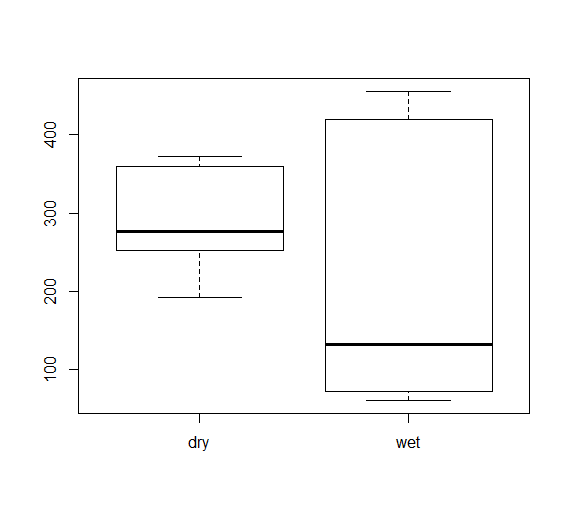
\includegraphics[scale=0.2]{../results/BoxHoursHum.png} }
          \subfigure[Environment]
          {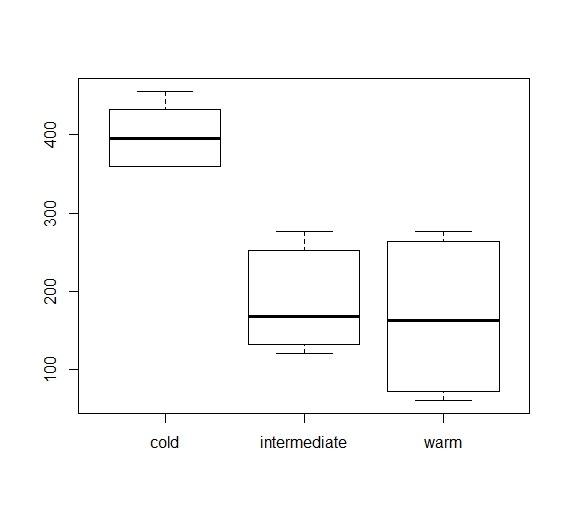
\includegraphics[scale=0.2]{../results/BoxHoursEnv.png} }
          \caption{Boxplots of Hours with Humidity and Environment}
          \label{fig:BoxHours}
      \end{figure} 
    
    \subsection*{3}
      \begin{figure}[H]
          \centering
          \subfigure[Humidity]
          {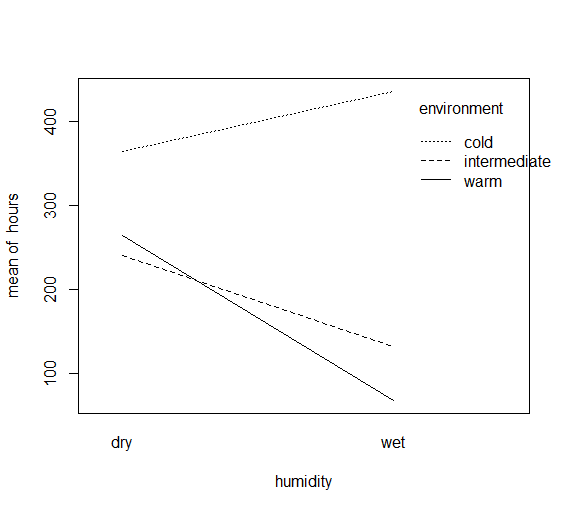
\includegraphics[scale=0.2]{../results/IntPlotHoursHum.png} }
          \subfigure[Environment]
          {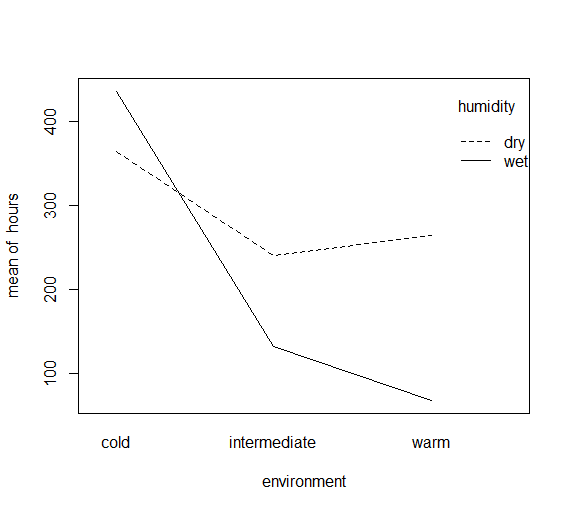
\includegraphics[scale=0.2]{../results/IntPlotHoursEnv.png} }
          \caption{Interactionplots of Hours with Humidity and Environment}
          \label{fig:IntPlotHours}
      \end{figure}
    
    \subsection*{4}
      Analysis of variance on both factors:\\\\
      \begin{lstlisting}[language=R]
Analysis of Variance Table

Response: hours
            Df Sum Sq Mean Sq F value    Pr(>F)    
environment  2 201904  100952 23.1057 3.674e-05 ***
humidity     1  26912   26912  6.1596   0.02637 *  
Residuals   14  61168    4369                      
---
Signif. codes:  0 ‘***’ 0.001 ‘**’ 0.01 ‘*’ 0.05 ‘.’ 0.1 ‘ ’ 1
      \end{lstlisting}
    
    \subsection*{5}
    
    \subsection*{6}
    
    \subsection*{7}
    
    \subsection*{8}
    
  \section*{Exercise 2}
    \subsection*{1}
     
    \subsection*{2}
    
    \subsection*{3}
    
    \subsection*{4}
    
    \subsection*{5}
    
    \subsection*{6}
    
    \subsection*{7}
    
  \section*{Exercise 3}
    \subsection*{1}
    
    \subsection*{2}
    
    \subsection*{3}
    
    \subsection*{4}
    
    \subsection*{5}
    
  \section*{Exercise 4}
    \subsection*{1}
    
    \subsection*{2}
    
    \subsection*{3}
    
    \subsection*{4}

    
  \section{R-Code}
    \subsection{Exercise 1}\label{sec:RE1}
      \begin{lstlisting}[language=R]
      \end{lstlisting}
    \subsection{Exercise 2}\label{sec:RE2}
      \begin{lstlisting}[language=R]
      \end{lstlisting}
    \subsection{Exercise 3}\label{sec:RE3}
      \begin{lstlisting}[language=R]
      \end{lstlisting}
    \subsection{Exercise 4}\label{sec:RE4}
      \begin{lstlisting}[language=R]
      \end{lstlisting}
\end{document}
